Substituting numerical values in 
	\eqref{eq:chapters/11/11/1/mat-3},
\begin{align}
 \myvec{6 & -14 & 1 \\
	12 & -12 & 1 \\
	6 & 6 & 1
	} \myvec {\vec{u} \\
	           f 
		}  = \myvec{-58 \\ -72 \\ -18 }
\end{align}
yielding
\begin{align}
	\vec{u} = \myvec{-3 \\ 2} \\ 
	f = -12 
\end{align}
See \figref{fig:10/7/4/3Fig1}.
\begin{figure}[H]
	\begin{center}
		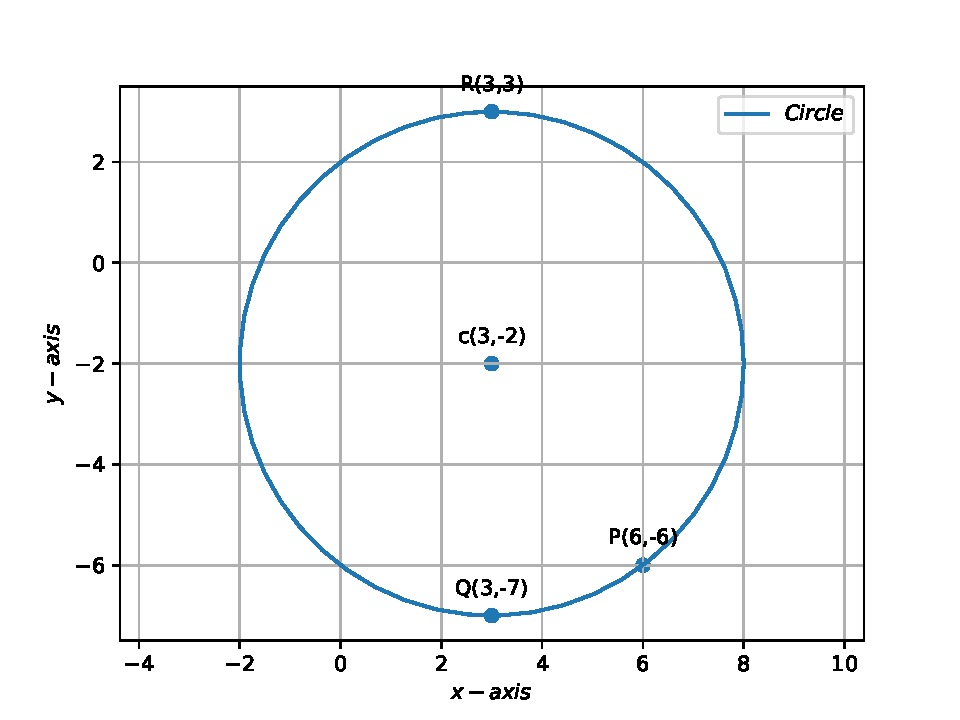
\includegraphics[width=0.75\columnwidth]{chapters/10/7/4/3/figs/problem3.pdf}
	\end{center}
\caption{}
\label{fig:10/7/4/3Fig1}
\end{figure}
